\section{Multilayer Perceptron}
\label{sec:mlp}

Advancements in the field of deep learning over the past decade have underscored the superiority of convolutional
and recurrent neural networks over traditional feedforward architectures, such as the \glsfirst{mlp}.\\
This superiority largely stems from CNNs' and RNNs' inherent abilities to capture spatial and temporal dependencies within
data.
Additionally, both CNNs and RNNs employ parameter sharing mechanisms -- across space for CNNs, and across time for \glspl{rnn}
-- decreasing their susceptibility to overfitting.\\

Nonetheless, the \gls{mlp} remains a foundational architecture worth exploring. This is especially true for tasks of low
complexity, where the risk of overfitting is low and the data not inherently spatially or temporally dependent.\\
However, the \gls{mlp} architecture has not been explored as extensively as the \gls{cnn} and \gls{rnn} architectures, and
is mostly an analogue to the previously introduced \gls{cnn} architecture.\\
Hence, the deep feed forward architecture will be a composite of \texttt{MLPBlock}s, each consisting of a linear layer,
followed by a normalization layer, a non-linear activation function, and finally a dropout layer. \\

\subsection{Hyperparameter Optimization}


\subsubsection{Number of Features}
\begin{figure}[H]
    \centering
    \subfloat[\texttt{MLPBlock 1}]{{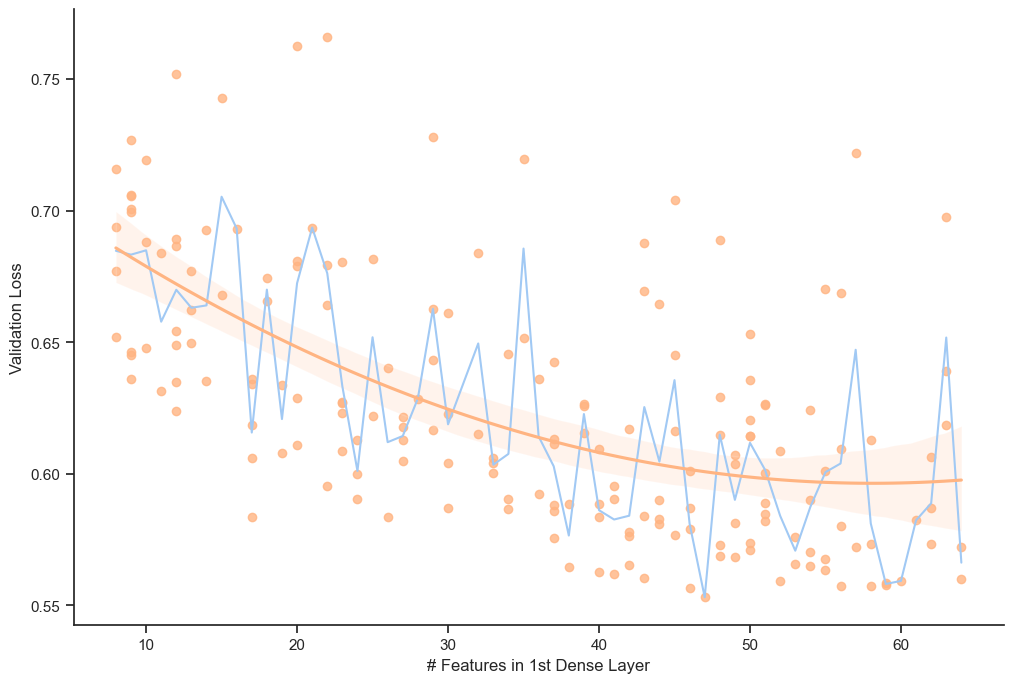
\includegraphics[width=0.33\textwidth]{figures/06_ModelExploration/5_MLP/ch1.png
    }}}
    \subfloat[\texttt{MLPBlock 2}]{{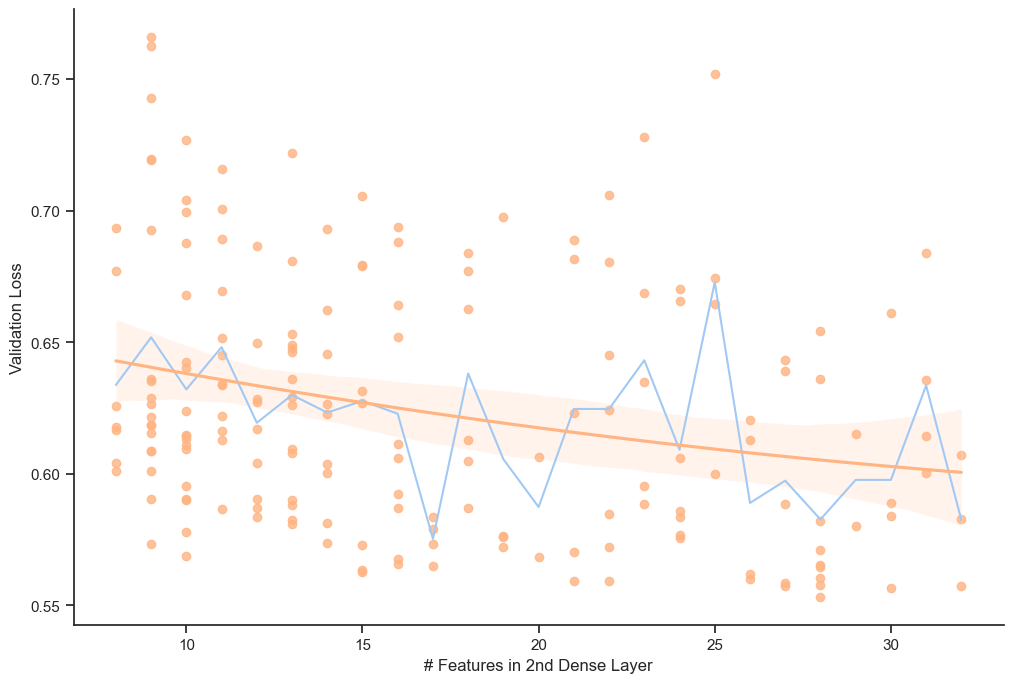
\includegraphics[width=0.33\textwidth]{figures/06_ModelExploration/5_MLP/ch2.png
    }}}
    \subfloat[\texttt{MLPBlock 3}]{{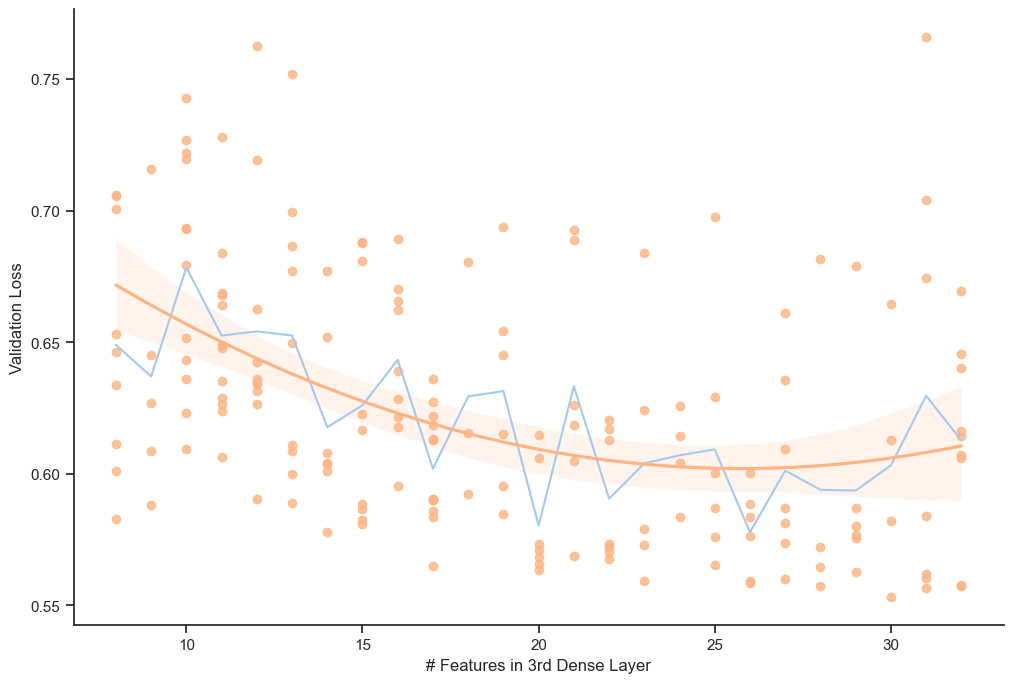
\includegraphics[width=0.33\textwidth]{figures/06_ModelExploration/5_MLP/ch3.png
    }}}
    \caption{Regression plots of the \( \lossCEVal \) for different numbers of features in the three \texttt{MLPBlock}s.}
    \label{fig:mlp_features}
\end{figure}

The exploration of the optimal number of features in the \texttt{MLPBlock}s, as depicted in \autoref{fig:mlp_features},
revealed a monotonically decreasing trend in validation loss with an increase in feature numbers for the second block, while
the first and third blocks each exhibited a local optimum within the explored range. \\
This observation suggests a higher feature count could potentially enhance model performance.
However, considering the stronger relative influence of the number of features in the first and third layers, the
feature count for the second \texttt{MLPBlock} was set to a rather conservative value of 20, to mitigate model complexity and
potential overfitting.

In retrospect, this decision seems doubious, as the subsequent \texttt{MLPBlock} contains four more features than block
two. This might cause an unwanted bottleneck effect and make some information in the last block redundant.\\


\subsubsection{Normalization and Residual Connection}

\begin{table}[H]
    \centering
    \caption{Comparison of MLP Variants}
    \label{tab:mlp_variants}
    \begin{tabular}{@{}lccccc@{}}
    \toprule
    Configuration & \multicolumn{2}{c}{\( \meanLossCEVal \)} & \multicolumn{2}{c}{\( \meanAccVal \)} \\
    \cmidrule(lr){2-3} \cmidrule(lr){4-5}
                  & \( \nu \) & \( \%\Delta \) & \( \nu \) & \( \%\Delta \) \\
    \midrule
    \multicolumn{5}{l}{Normalization} \\
    False          & 0.657 & - & 0.696 & - \\
    Batch Norm     & 0.656 & \gnbx{-0.208} & 0.706 & \gnbx{1.429} \\
    Instance Norm  & 0.621 & \gnbx{-5.567} & 0.717 & \gnbx{3.011} \\
    Layer Norm     & 0.596 & \gnbx{-9.245} & 0.728 & \gnbx{4.594} \\
    \midrule
    \multicolumn{5}{l}{Skip Connection} \\
    False          & 0.657 & - & 0.695 & - \\
    Skip           & 0.611 & \gnbx{-7.078} & 0.723 & \gnbx{4.067} \\
    \bottomrule
    \end{tabular}
\end{table}


The examination of normalization methods and skip connections within the MLP architecture reveals that both modifications
significantly influence model performance.\\
Normalization, particularly Layer Norm, markedly enhances model accuracy and reduces validation loss,
highlighting its role in stabilizing the training process and improving generalization.
Since the \gls{mlp}'s internal tensors do not exhibit separate spacial or temporal dimensions together with a channel
dimension, Instance Norm and Batch Norm aggregate their statistics in the same manner. Their difference lies in the
subsequent scaling and shifting operations.\\
While Layer Norm uses individual scaling and shifting parameters (\( \bfm{\gamma}, \bfm{\beta} \)) for each feature,
it was not possible to instantiate Instance Norm with the inclusion of the subsequent affine transformation.

The integration of skip connections also shows a notable positive effect on the model's performance.
The linear transformation within the skip branch, designed to align the feature count with the final \texttt{MLPBlock}, is then
added to the last \texttt{MLPBlock}'s output.
This addition introduces only a marginal increase in model complexity, with \( 9 \times ( 24 + 1) = 225 \) additional parameters.\\


\subsection{Resulting Architecture}
\label{sub:mlp_architecture}

The \gls{mlp} model used for testing and final comparative analysis is visualized in \autoref{fig:mlp_model}.\\
Unfortunately, the skip connection, which is highlighted in purple in the diagram, was not implemented into the final model as initially intended.

\begin{figure}[H]
    \centering
    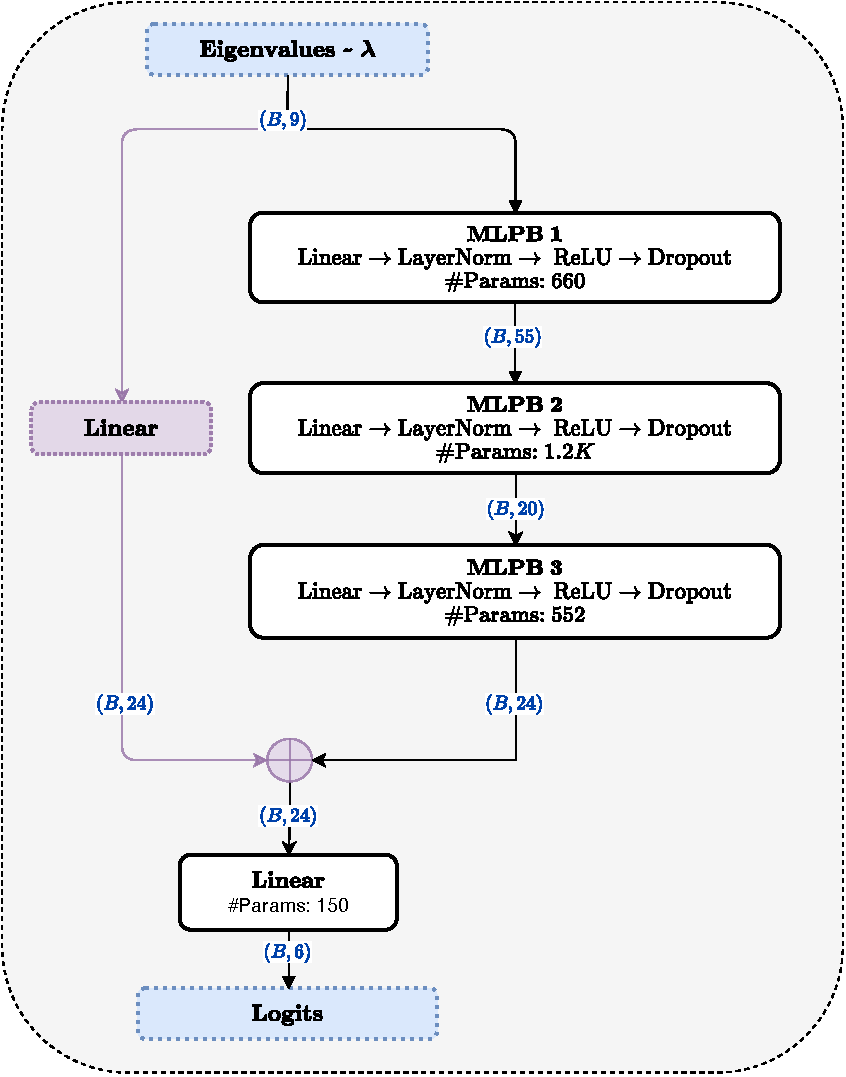
\includegraphics[width=0.45\textwidth]{figures/06_ModelExploration/mlp.pdf}
    \caption{Flowchart of the MLP architecture.}
    \label{fig:mlp_model}
\end{figure}

The architecture, as depicted, encapsulates a sequential arrangement of three \texttt{MLPBlock}s, each comprising essential
components for a feedforward network: linear transformation, normalization, activation, and regularization through
dropout.\\

\autoref{tab:mlp_summary} summarizes the hyperparameters and layer configurations of the final \gls{mlp} model.

\begin{table}
    \centering
    \caption{Summary of Hyperparameters and Layer Configurations for DenseNet}
    \label{tab:mlp_summary}
    \small
    \begin{tabular}{@{}lll@{}}
    \toprule
    \textbf{Block / Module}               & \textbf{Child}        & \textbf{Parameters / Value}            \\ \midrule
    \multicolumn{3}{l}{\textbf{Modules}}                                                     \\ \midrule
    \multirow{7}{*}{\texttt{MLPBlock} 1} & \texttt{nn.Linear}           & Features: \(9 \rightarrow 55\) \\
                                         &                              & \#Params \( = 9 \times 55 + 55 = 550\) \\
                                         & \texttt{nn.LayerNorm}        & \#Params \( = 2 \times 55 = 110\) \\
                                         & \texttt{nn.ReLU}             & \\
                                         & \texttt{nn.Dropout}          & Rate: 0.06                      \\
                                         & \( \Sigma \) \#Params        & 660 \\ \midrule
    \multirow{6}{*}{\texttt{MLPBlock} 2} & \texttt{nn.Linear}           & Features: \(55 \rightarrow 20\) \\
                                         &                              & \#Params \( = 55 \times 20 + 20 = 1120\) \\
                                         & \texttt{nn.LayerNorm}        & \#Params \( = 2 \times 20 = 40\) \\
                                         & \texttt{nn.ReLU}             & \\
                                         & \texttt{nn.Dropout}          & Rate: 0.06                      \\
                                         & \( \Sigma \) \#Params        & 1160 \\ \midrule
    \multirow{6}{*}{\texttt{MLPBlock} 3} & \texttt{nn.Linear}           & Features: \(20 \rightarrow 24\) \\
                                         &                              & \#Params \( = 20 \times 24 + 24 = 504\) \\
                                         & \texttt{nn.LayerNorm}        & \#Params \( = 2 \times 24 = 48\) \\
                                         & \texttt{nn.ReLU}             & \\
                                         & \texttt{nn.Dropout}          & Rate: 0.06                      \\
                                         & \( \Sigma \) \#Params               & 552 \\ \midrule
    Head                                 & \texttt{nn.Linear}           & \#Params \( = 24 \times \| \NSet \| + \| \NSet \| = 150\) \\
                                         &                              & \#Params = 150 \\
    \midrule[0.1pt]
    \addlinespace[0.5cm]
    \( \Sigma \) \#Params                & \texttt{DenseNet} & 2522 \\
    \bottomrule

    \addlinespace[1cm]
    \multicolumn{3}{l}{\textbf{Non-Layer Hyperparameters}}                                       \\ \midrule
    Optimizer                            &                           & \texttt{optim.AdamW} \\
    Batch Size                           &                           & 512                       \\
    Learning Rate                        &                           & 0.005                     \\
    Weight Decay                         &                           & 0.01685                   \\
    LR Scheduler                         &                           & \texttt{lr\_scheduler.ReduceLROnPlateau}\\
    Precision                            &                           & \texttt{32bit-true}     \\
    \bottomrule
    \end{tabular}
\end{table}

Without any further hyperparameter optimization, the learning rate of the final model was set to a value of
\( \alpha = 0.005 \)%
\footnote{Retrospectively, this value seems to be too high, as argumented in~\autoref{subsub:considerations_nn}.}.
The weight decay, as well as the dropout rate have been adapted from the convolutional model.\\

\subsubsection{Future Improvements}

Given the freedom of choice with respect to the number of features in the \texttt{MLPBlock}s, an adaptation worth considering
would be to align the feature count in the second \texttt{MLPBlock} to match the third could mitigate potential information
bottlenecking and enable the model to leverage a broader feature representation. This adjustment might not only harmonize
the flow of information across the layers but could also pave the way for implementing a true residual connection,
paralleling the final \texttt{MLPBlock}, to further enhance the model's learning capacity without substantially increasing its complexity.

Should the model be considered for further development, it would also be interesting to explore the impact of pruning
techniques on the model's performance.\\

The observed slight performance improvements through the use of \gls{prelu} over \gls{relu} in the convolutional model
suggest that these findings could be transferred to the \gls{mlp} model.\\

Moreover, considering the future development of the model, the application of pruning techniques could be investigated
to refine the network's architecture by identifying and eliminating redundant units or connections, thereby streamlining
the model for improved efficiency.
